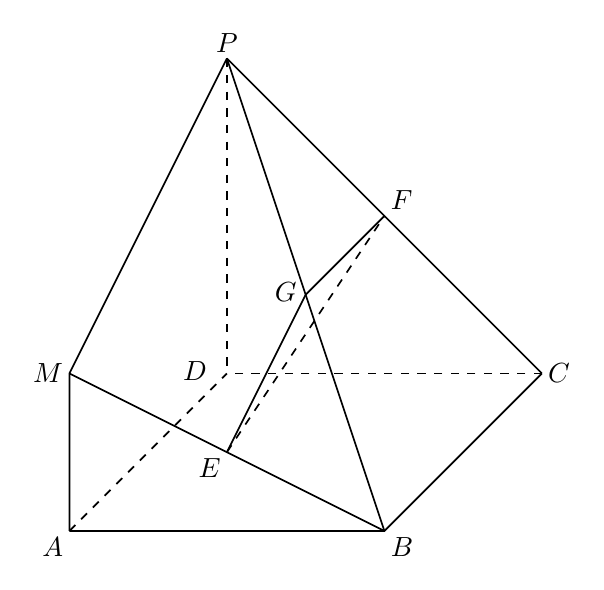
\begin{tikzpicture}[x=1cm,y=1cm,line width=.6pt,font=\normalsize,
  geometry edge/.style={solid,line width=.6pt},
  geometry label/.style={font=\normalsize,inner sep=2pt}]
\coordinate (A) at (0,0);
\coordinate (B) at (4,0);
\coordinate (C) at (6,2);
\coordinate (D) at (2,2);
\coordinate (M) at (0.0000000000,2.0000000000);
\coordinate (P) at (2,6);
\coordinate (E) at (2.0000000000,1.0000000000);
\coordinate (G) at (3.0000000000,3.0000000000);
\coordinate (F) at (4.0000000000,4.0000000000);
\draw[geometry edge] (A)--(B)--(C);
\draw[geometry edge,dashed] (C)--(D);
\draw[geometry edge,dashed] (A)--(D);
\draw[geometry edge] (A)--(M)--(P);
\draw[geometry edge] (M)--(B);
\draw[geometry edge] (P)--(B);
\draw[geometry edge] (P)--(C);
\draw[geometry edge,dashed] (P)--(D);

\draw[geometry edge] (E)--(G);
\draw[geometry edge] (G)--(F);
\draw[geometry edge,dashed] (E)--(F);

\node[geometry label,below left] at (A) {$A$};
\node[geometry label,below right] at (B) {$B$};
\node[geometry label,right] at (C) {$C$};
\node[geometry label,above left,xshift=-5pt,yshift=-5pt] at (D) {$D$};
\node[geometry label,left] at (M) {$M$};
\node[geometry label,above] at (P) {$P$};
\node[geometry label,below left] at (E) {$E$};
\node[geometry label,left,xshift=-1pt,yshift=1pt] at (G) {$G$};
\node[geometry label,above right] at (F) {$F$};
\end{tikzpicture}
